\documentclass[notes]{subfiles}
\begin{document}
	\addcontentsline{toc}{section}{2.3/4.6 - Limit Laws \& Limits at Infinity}
	\refstepcounter{section}
	\fancyhead[RO,LE]{\bfseries \nameref{cs23}} 
	\fancyhead[LO,RE]{\bfseries \small \currentname}
	\fancyfoot[C]{{}}
	\fancyfoot[LO,RE]{\large \thepage}	%Footer on Right \thepage is pagenumber
	\fancyfoot[RO,LE]{\large Chapter 2.3/4.6}

\section*{Limit Laws \& Limits at Infinity}\label{cs23}
	\subsection*{Before Class}
	\subsubsection*{The Limit Laws}
		\begin{thm}[Limit Laws]
			Suppose that \(c\) is a constant, and that the limits \(\ds \lim_{x\to a} f(x)\) and \(\ds \lim_{x\to a} g(x)\) exist. Then,
			\\ \\
				\begin{enumerate}
					\setlength\itemsep{40pt}
					\item 
					\item 
					\item 
					\item 
					\item 
					\item 
					\item 
				\end{enumerate}
		\end{thm}
			\newpage

		\begin{ex}
			Use the limit laws to determine the following limits, if they exist.  The function \(f(x)\) is graphed as the solid line, and \(g(x)\) is graphed as the dashed line.\\[10pt]
			\begin{minipage}{.38\textwidth}
				\begin{flushleft}
					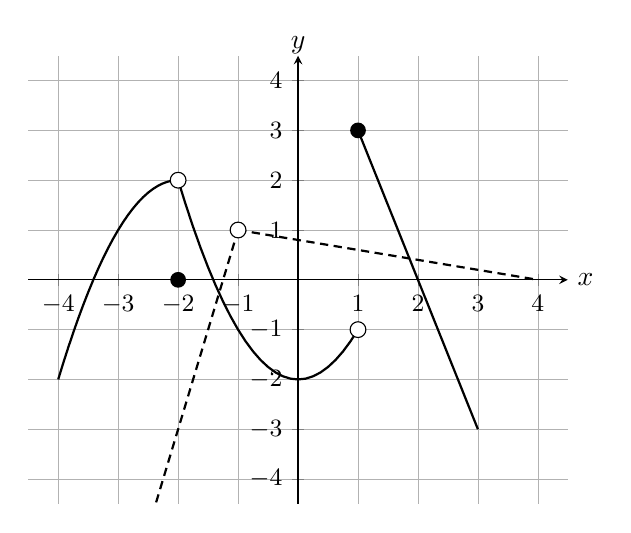
\begin{tikzpicture}
						\begin{axis}[
							grid style = {line width = .1pt, draw = gray!60},
							grid = both,
							every tick label/.append style={font=\small},
							axis x line = middle,
							axis y line = middle,
				    			every axis y label/.style={at={(ticklabel cs:1.15)}, yshift = -3pt},
								y label style={at={(axis description cs: 0.5, 1)},above},
							ytick = {-4,-3,-2,-1,1,2,3,4},
				    			ylabel = {$y$},
				    			ymin = -4.5, ymax = 4.5,
			    				every axis x label/.style= {at ={(ticklabel cs:1)}},
			    				xtick = {-4,-3,-2,-1,1,2,3,4},
				    				x label style={at={(axis description cs: 1, 0.5)},right},
			    				xlabel = {$x$},
			    				xmin = -4.5, xmax = 4.5			
						]	
							\addplot[thick, domain = -4:-2] {-(x+2)^2+2};
								\coordinate (circle1) at (-2,2);
								\coordinate (circle4) at (-2,0);
							\addplot[thick, domain = -2:1] {x^2-2};
							\addplot[thick, densely dashed, domain = -2.5:-1] {4*x+5};
								\coordinate (circle2) at (-1,1);
							\addplot[thick, densely dashed, domain = -1:4] {-.2*x+.8};
							\addplot[thick, domain = 1:3] {-3*x+6};
								\coordinate (circle3) at (1,3);
								\coordinate (circle5) at (1,-1);
						\end{axis}
							\fill[white] (circle1) circle (.1);
							\draw (circle1) circle (0.1);
							\fill (circle4) circle (0.1);
							\fill[white] (circle2) circle (0.1);
							\draw (circle2) circle (0.1);
							\fill[white] (circle5) circle (0.1);
							\draw (circle5) circle (0.1);
							\fill (circle3) circle (0.1);
					\end{tikzpicture}
				\end{flushleft}
			\end{minipage} \hspace{15pt}
			\begin{minipage}{.58\textwidth}
				\begin{flushleft}
					\begin{multicols*}{2}
						\begin{enumerate}[(a)]
							\item \(\ds \lim_{x\to 1} [f(x)]\)
								\vspace{1in}
							\item \(\ds \lim_{x\to -1} [g(x)]\)
								\vspace{1in}
							\item \(\ds \lim_{x\to -2}\left[\dfrac{f(x)}{g(x)}\right]\)
								\vspace{1in}
								\columnbreak 
							\item \(\ds \lim_{x\to -1}\left[f(x)g(x)\right]\)
								\vspace{1in}
							\item \(\ds \lim_{x\to -1}\left[-2f(x)+3g(x)\right]\)
								\vspace{1.1in}
							\item \(\ds \lim_{x\to 2} [3f(x)]\)
								\vspace{1in}
						\end{enumerate}
							\raggedcolumns
					\end{multicols*}
				\end{flushleft}
			\end{minipage}
		\end{ex}
			\vs{1}

		\begin{ex}
			Assume that \(\ds \lim_{x\to 3} f(x) = -1\), \(\ds \lim_{x\to 3} g(x) = 2\), and \(\ds \lim_{x\to 3} h(x) = 0\).  Find the following limits, if they exist.  If they don't, explain why.  Justify each answer with the appropriate limit law(s).
			\begin{enumerate}[(a)]
				\item \(\ds \lim_{x\to 3} [f(x) + 5g(x)]\)
					\vs{1}
				\item \(\ds \lim_{x\to 3} [f(x)]^5\)
					\vs{1}
				
				\item \(\ds \lim_{x\to 3} \sqrt{g(x)}\)
					\vs{1}
					\newpage

				\item \(\ds \lim_{x\to 3} \dfrac{3f(x)}{g(x)}\)
					\vs{1}
					
				\item \(\ds \lim_{x\to 3} \dfrac{g(x)}{h(x)}\)
					\vs{1}
					
				\item \(\ds \lim_{x\to 3} \dfrac{f(x)h(x)}{g(x)}\)
					\vs{1}			
			\end{enumerate}
		\end{ex}

	\subsubsection*{Evaluating Limits}
		\begin{rmk}[Direct Substitution Property]
			If \(f\) is a  function with \(a\) in its domain, then 
				\\ \\ \\
		\end{rmk}	

		\begin{ex}
			Calculate the following limits.  Justify each answer with one (or more) of the limit laws.
			\begin{enumerate}[(a)]
				\item \(\ds \lim_{x\to -1} 3x^3+5x^2-7\)
					\vs{1}
					\newpage
					
				\item \(\ds \lim_{x\to 2} \dfrac{x^3+2x^2-1}{5-3x}\)
					\vs{1}
					
				\item \(\ds \lim_{x\to 1} \dfrac{x-1}{x^2+1}\)
					\vs{1}
					
			\end{enumerate}
		\end{ex}

		\begin{question}
			Let \(k(x) = \dfrac{x+1}{x^2-1}\).
			\begin{enumerate}[(a)]
				\item The Direct Substitution Property \emph{cannot} be applied to the function at \(x = -1\).  Why not?
					\vs{1}
					
				\item Modify the function so that you \emph{can} use the Direct Substitution Property.
					\vs{1}
			\end{enumerate}
		\end{question} 
			\newpage
			
	\subsubsection*{Limits at Infinity}
		\begin{defn}[Limits at Infinity]
			Let \(f\) be a function defined on some interval \((a,\infty)\).  Then

					\\[40pt] \(\) \\
				
			means that the values of \(f(x)\) can be made arbitrarily close to \(L\) by requiring \(x\) to be sufficiently large.  If \(g\) is defined on some interval \((-\infty,a)\), then
					\\[50pt] \(\) \\
			means that the values of \(g(x)\) can be made arbitrarily close to \(L\) by requiring \(x\) to be sufficiently large negative.
		\end{defn}
			
		We read the limits above (for \(f\)) as
			\begin{itemize}
			\setlength\itemsep{40pt}
				\item 
				\item 
			\end{itemize}
			\vspace*{.1in}
		with the obvious changes for \(g\). 

		\begin{defn}[Horizontal Asymptote]
			The line \(y = L\) is called a \textbf{horizontal asymptote} of the curve \(y = f(x)\) if either 
				\vspace{.75in}
		\end{defn}
			\newpage
			
		\begin{ex}
			Write the horizontal asymptotes of the function \(f(x) = \dfrac{x^2-1}{x^2 + 1}\)
		\end{ex}
			\vs{1}

		\begin{ex}
			The function \(f(x) = \dfrac{x-9}{\sqrt{4x^2 + 3}}\) has two horizontal asymptotes; find them, and express the asymptotes using limit notation.
		\end{ex}
			\vs{2}
		
			\newpage
			
	\subsection*{Pre Class Practice}
		\begin{ex}
			Compute the following limits:
			\begin{enumerate}[(a)]
				\item \(\ds \lim_{x\to 0} (4x^2-2x+3)\)
					\vs{1}
					
				\item \(\ds \lim_{x\to 2} (e^{2x-x^2})\)
					\vs{1}
					
				\item \(\ds \lim_{t\to 1} \dfrac{2-7t}{t+6}\)
					\vs{1}
					
				\item \(\ds \lim_{x\to 3} (\ln (e^{3x}))\)
					\vs{1}
			\end{enumerate}
		\end{ex}
			\newpage
			
		
		\begin{ex}
			Use the graph to compute the limits. \(f(x)\) is given by the solid lines, and \(g(x)\) by the dotted lines.
			\begin{center}
				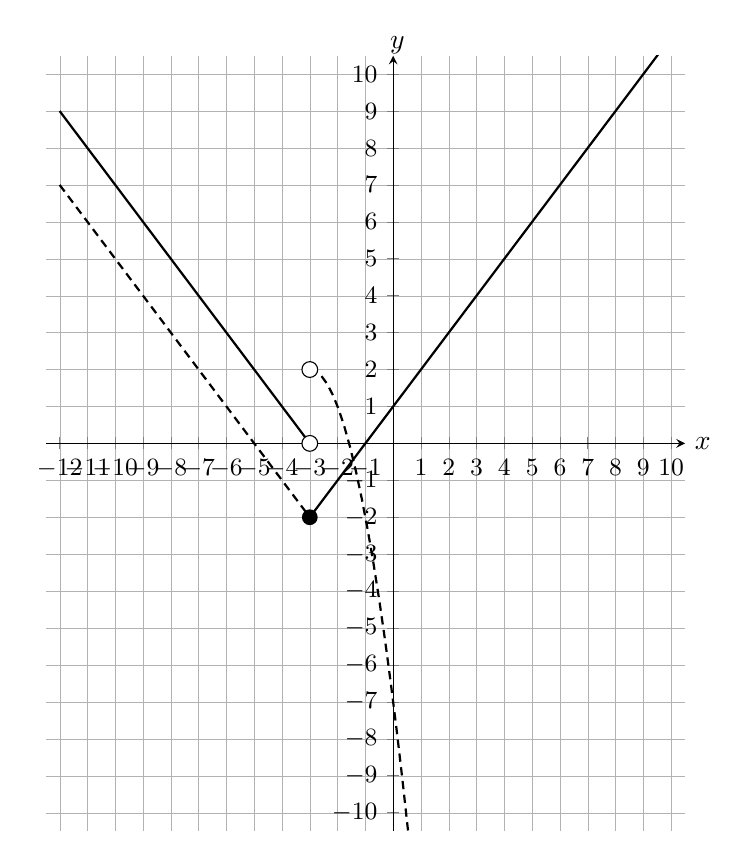
\begin{tikzpicture}
						\begin{axis}[
							grid style = {line width = .1pt, draw = gray!60},
							grid = both,
							width = .8\textwidth,
							height = 4.5in,
							every tick label/.append style={font=\small},
							axis x line = middle,
							axis y line = middle,
				    			every axis y label/.style={at={(ticklabel cs:1.15)}, yshift = -3pt},
								y label style={at={(axis description cs: 0.55, 1)},above},
							ytick = {-10,...,10},
				    			ylabel = {$y$},
				    			ymin = -10.5, ymax = 10.5,
			    				every axis x label/.style= {at ={(ticklabel cs:1)}},
			    				xtick = {-12,...,10},
				    				x label style={at={(axis description cs: 1, 0.5)},right},
			    				xlabel = {$x$},
			    				xmin = -12.5, xmax = 10.5			
						]	
							\addplot[thick, domain=-12:-3] {-x-3};
								\coordinate (a) at (-3,0);
							\addplot[thick, domain=-3:10] {x+1};
								\coordinate (b) at (-3,-2);
							\addplot[thick, densely dashed, domain=-12:-3] {-x-5};
							\addplot[thick, densely dashed, domain=-3:2] {-(x+3)^2 + 2};
								\coordinate (c) at (-3,2);
						\end{axis}
							\fill[white] (a) circle (0.1);
							\draw (a) circle (0.1);
							\fill (b) circle (0.1);
							\fill[white] (c) circle (0.1);
							\draw (c) circle (0.1);
							
					\end{tikzpicture}
			\end{center}
			\begin{minipage}{1.3\textwidth}
				\begin{multicols*}{2}
				\begin{enumerate}[(a)]
					\setlength{\itemsep}{2in}
					\item \(\ds \lim_{x\to -3} 2g(x)\)
						
					\item \(\ds \lim_{x\to 0} \sqrt{f(x) -g(x)}\)
						
					\item \(\ds \lim_{x\to -5} \dfrac{g(x) + 1}{3f(x)}\)
						
					\item \(\ds \lim_{x\to -2} (f(x) + g(x))^2\)

				\end{enumerate}
					\raggedcolumns
				\end{multicols*}
			\end{minipage}
		\end{ex}
			\newpage
			
	\subsection*{In Class}
	\subsubsection*{Examples}
		\begin{ex}
			Compute the following limits:
			\begin{enumerate}[(a)]
				\item \(\ds \lim_{t\to -5} g(t)\), where \(g(t) = \begin{cases}t^2 -1 & t\neq -5\\ \pi+1 & t = -5 \end{cases}\)
					\vs{1}
					
				\item \(\ds \lim_{h\to 0} \dfrac{f(x+h)-f(x)}{h}\), where \(f(x) = x^2+2x-1\)
					\vs{1}
					
				\item \(\ds \lim_{x\to -4} \dfrac{3x + 12}{|x + 4|}\)
					\vs{1}

				\item \(\ds \lim_{x\to 2} \dfrac{\sqrt{4x+1} - 3}{x-2}\)
					\vs{1}

			\end{enumerate}
		\end{ex}
			\newpage
		
		\begin{ex}
			Write the horizontal asymptotes of the function  \(f(x) =\dfrac{3x-2}{2x^2+1}\).
		\end{ex}
			\vs{1}
				
		\begin{ex}
			Does the function \(f(x) = \dfrac{1-x^3}{x^2-x+1}\) have any horizontal asymptotes?  If it does, give their equation.  If it doesn't, explain why.
		\end{ex}
			\vs{1}

		\begin{question}
			Think about \(\ds \lim_{x\to\infty} \dfrac{1}{x}\) and \(\ds \lim_{x\to -\infty} \dfrac{1}{x}\).  What do you expect these limits to be?\\[5pt]  Why?  What about \(\ds \lim_{x\to \pm \infty} x^r\), for some \(r > 0\)?
		\end{question}
			\vs{1}
			\newpage
			
		\begin{rmk}[Theorem]
			If \(r > 0\) is a rational number, then 
					\vspace{.75in} \\ \\
			If \(r > 0\) is a rational number such that \(x^r\) is defined for all \(x\), then
					\vspace{.75in}
		\end{rmk}
		
		\begin{ex}
			Evaluate \(\ds \lim_{x\to \infty} \dfrac{3x^2-x-2}{5x^2+4x+1}\)
		\end{ex}
			\vs{1.5}
			\newpage
			
		\begin{ex}
			Find the asymptotes of \(f(x) = \dfrac{\sqrt{2x^2+1}}{3x-5}\)
		\end{ex}
			\vs{1}
			
		\begin{ex}
			Compute \(\ds \lim_{x\to \infty} (\sqrt{x^2+2}-x)\)
		\end{ex}
			\vs{1}
			\newpage
		\begin{ex}
			Find the following limits, or argue why it doesn't exist:
			\begin{enumerate}[(a)]
				\item \(\ds \lim_{x\to -\infty} \dfrac{4x^3 + 6x^2 - 2}{2x^3 - 4x + 5}\)
					\vs{1}
					
				\item \(\ds \lim_{x\to -\infty} \dfrac{\sqrt{1+4x^6}}{2-x^3}\)
					\vs{1}
					
				\item \(\ds \lim_{x\to \infty} e^x\)
					\vs{1}
					
			\end{enumerate}
		\end{ex}		
			\newpage
			
	\subsection*{After Class Practice}
		\begin{ex}
			The \emph{signum function} (or the \emph{sign function}), \(\text{sgn}(x)\), is given by \[\text{sgn}(x) = \begin{cases}-1 & x < 0\\ 0 & x = 0\\ 1 & x > 0 \end{cases}\]  
			\begin{enumerate}[(a)]
				\item Sketch the graph of \(\text{sgn}(x)\).
					\vs{1}
					
				\item Find the limits, or explain why they don't exist:
					\begin{enumerate}[(a)]
						\item \(\ds \lim_{x\to 0} \text{sgn}(x)\)
							\vs{.5}
						\item \(\ds \lim_{x\to 0} |\text{sgn}(x)|\)
							\vs{.5}
					\end{enumerate}
			\end{enumerate}
		\end{ex}
		
		\begin{ex}
			Compute the limits:
			\begin{enumerate}[(a)]
				\item \(\ds \lim_{h\to 0} \dfrac{f(1+h)-f(1)}{h}\), where \(f(x) = \sqrt{x}\)
					\vs{1}
					
				\item \(\ds \lim_{x\to -1} \dfrac{2x^2 + 3x + 1}{x^2 - 2x -3}\)
					\vs{1}
					\newpage
					
				\item \(\ds \lim_{h\to 0} \dfrac{(x+h)^3 - x^3}{h}\)
					\vs{1}
					
				\item \(\ds \lim_{x\to \infty} \lrpar{\sqrt{9x^2 + x} - 3x}\)
					\vs{1}
					
				\item \(\ds \lim_{x\to \infty} \sqrt{x^2 + 2}\)
					\vs{1}
			\end{enumerate}
		\end{ex}
\clearpage
\end{document}
